\todo{Comm Gateway beschreiben}

\subsubsection{Mailbox Kommunikation ARM $\leftrightarrow$ NIOS2}
Die Kommunikation über die in das \ac{FPGA} programmierte Mailbox (siehe \ref{IP-Cores}) wird über eine abstrakte Klassenimplementierung in C++ dargestellt. \todo{Name, Pfad?}
Die Klasse stellt einige \textit{Write} und \textit{Read} Funktionen zur Verfügung, die mit verschiedenen Objekten umgehen können. Durch dieses Vorgehen ist sichergestellt, das der Aufrufer als Übergabeparameter nur bestimmte Objekte (die sauber definiert sind) übergegeben werden können, die auch verarbeitet werden können. Die Kommunikation erfolgt asynchron und ist intern gepuffert. Die Klasse dient als Abstraktionsschicht in beide Richtungen. Sowohl die Empfangsrichtung als auch die Senderichtung werden über die Klasse abgebildet, sodass der Aufrufer keinerlei interne Informationen über die Hardware und die Implementierung haben muss.
Nachfolgend werden die beiden wesentlichen Operationen (\textit{Write} und \textit{Read}) dargestellt und beschrieben.

\begin{figure}
	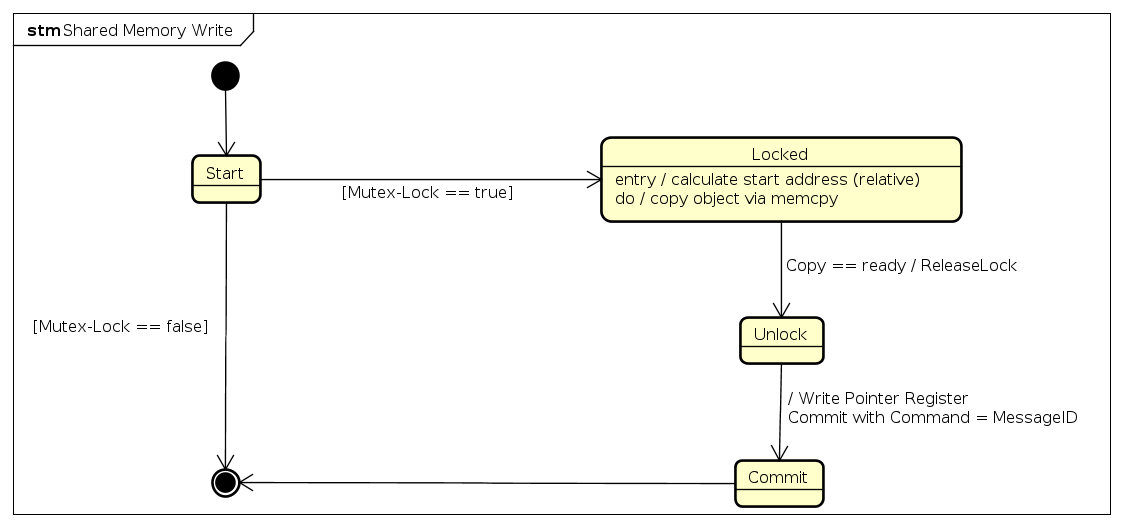
\includegraphics[width=\textwidth]{Abb/Shared_mem_Write.png}
	\caption{Schreibvorgang in den Shared Memory}
	\label{Software:Arm:SharedMemWrite}
\end{figure}

\paragraph{Write}
Der schreibende Zugriff auf den Shared Memory ist in Abbildung \ref{Software:Arm:SharedMemWrite} illustriert und hat einen einfachen Ablauf. Nachdem sich der Schreiber den Lock auf den Shared Memory über den Mutex Core geholt hat kann er Daten in diesen Bereich schreiben. Der Speicher wird dabei linear durchlaufen. Der Speicher wird dabei wie ein Ringspeicher behandelt. Ist am oberen Ende des Speichers nicht mehr genug Platz für die neue Nachricht wird wieder bei der relativen Addresse Null angefangen zu schreiben. Sind alle Daten in den Speicher geschrieben wird der Mutex wieder freigelassen. Im Speicher steht jetzt ein Abbild des Objekts, das übertragen werden soll. Es werden also nur Nutzdaten in den Speicher geschrieben. Anschließend wird die Startaddresse der Daten in das Pointer Register der Mailbox geschrieben. In das Command Register wird die eindeutige Nachrichten ID, die innerhalb des Garfield Projekts definiert ist, geschrieben. Dieser Schreibvorgang ist die letzte Instruktion zum Nachrichtenaustausch aus Sendersicht.

\paragraph{Read}
Der lesende Zugriff auf den Shared Memory ist komplizierter und unterteilt sich in zwei Abschnitte.\\

Der erste Teil der lesenden Kommunikation besteht aus dem \textbf{Interrupt}. Von dem Mailbox \ac{IP}-Core wird bei einem schreibenden Zugriff auf das Command Register automatisch ein Interrupt erzeugt. Innerhalb des \textit{ReadInterruptHandler} wird nicht der Shared Memory ausgelesen, sondern nur die Nachricht aus der Mailbox gespeichert. Die Klasse hält zusätzlich zu jedem Objekt, das verschickt bzw. empfangen werden soll einen kleinen Ringpuffer. Dieser dient dazu, die Addressen der Objekte im Shared Memory zu puffern. Tritt nun das Interrupt auf, wird zuerst das Pointer Register zwischengespeichert. Anschließend wird das Command Register, in dem der Nachrichtentyp übertragen wird, ausgelesen und anhand des Nachrichtentyps die Addresse des Pointer Registers in den passenden Puffer geschrieben. Dieses Vorgehen sorgt dafür, dass diese Funktion, die in einem Interrupthandler ausgeführt wird, sehr schnell wieder beendet ist.\\

Der zweite Teil besteht aus einem \textbf{Hintergrundtask} der zyklisch durchlaufen wird. Innerhalb dieses Task werden die Werte eines Objekts, die ausgelesen werden sollen, über eine \textit{Read} Funktion bei Bedarf überschrieben. Bei Bedarf deswegen, weil die Werte nur überschrieben werden, wenn aktuellere Werte im Shared Memory stehen. Sind aktuelle Werte verfügbar, ist der Klasseninterne Ringpuffer, der die Addressen für die Nutzdaten enthält, nicht leer. Es wird über die Addresse aus dem Shared Memory gelesen und anschließend diese Nachricht (also die Addresse) aus dem Ringpuffer entfernt.